\documentclass[12pt]{article}

% Indent the first paragraph of a chapter/section
% Apparently this package just sets \@afterindentfalse to (always) true.
\usepackage{indentfirst}

% Non-terrible references
\usepackage{hyperref}

\usepackage{tikz}
\usetikzlibrary{positioning}
\tikzstyle{arrow} = [thick,->,>=stealth]

\begin{document}

\begin{center}
  \Large{\textbf{Intercept Compilation Overview}}

  \vspace{1ex}
  \large{From Source Code to Machine Code}

  \vspace{1ex}
  \textbf{Lens\_r}

  \noindent\rule{\textwidth}{0.4pt}
\end{center}

\section{Compilation Overview}
\label{sec:overview}

\begin{figure}[ht]
  \centering
  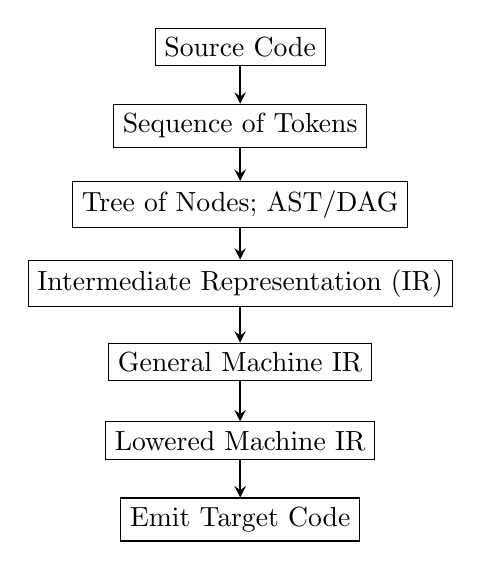
\begin{tikzpicture}
    \node (src) [draw] {Source Code};

    \node (tok) [draw, below of=src] at (0,0) {Sequence of Tokens}; % lex into tokens (skip whitespace/comments, interpret numbers, etc)
    \draw [arrow] (src) -- (tok);

    \node (ast) [draw, below of=tok] {Tree of Nodes; AST/DAG}; % parse into ast/dag, semantic analysis (type checking, program correctness, etc)
    \draw [arrow] (tok) -- (ast);

    \node (ir) [draw, below of=ast] {Intermediate Representation (IR)}; % codegen ast/dag into unlowered IR, optimise IR, *lower IR
    \draw [arrow] (ast) -- (ir);

    \node (gmir) [draw, below of=ir] {General Machine IR}; % lower IR into gMIR (near 1:1 mapping of IR), phi2copy, operand inlining
    \draw [arrow] (ir) -- (gmir);

    \node (lmir) [draw, below of=gmir] {Lowered Machine IR}; % ISel into lMIR, do register allocation for virtual registers
    \draw [arrow] (gmir) -- (lmir);

    \node (code) [draw, below of=lmir] {Emit Target Code}; % lMIR gets converted directly into target code (assembly, object file, etc)
    \draw [arrow] (lmir) -- (code);
  \end{tikzpicture}
  \caption{Steps of the compilation process implemented by Intercept}
\end{figure}

It should be noted that both general and lowered MIR are stored in the same data structure.

\section{Source Code}
\label{sec:source-code}

\par
This is what programmers will write, expecting this compiler to be able to turn it into target code.

\begin{figure}[ht]
  \centering
  foo :: 69; foo
  \caption{Source code of a very simple Intercept program}
  \label{fig:int-source}
\end{figure}

\section{Token Sequence}
\label{sec:tokens}

The source code is first split into lexemes, or tokens. Each of these tokens may have a both a number and/or a textual value associated with it. The act of splitting input into tokens like this is called \emph{lexing}.

\begin{figure}[ht]
  \centering
  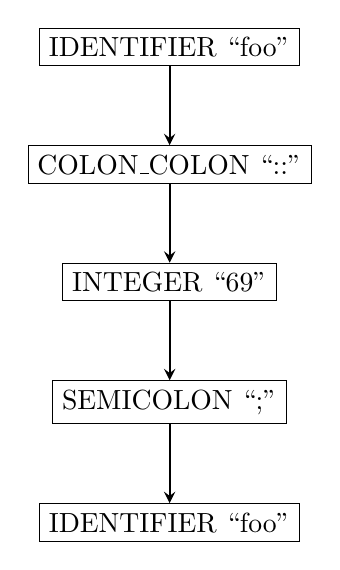
\begin{tikzpicture}
    \node (decl-id) [draw] {IDENTIFIER ``foo''};

    \node (decl-op) [draw, below=of decl-id] {COLON\_COLON ``::''};
    \draw [arrow] (decl-id) -- (decl-op);

    \node (decl-init) [draw, below=of decl-op] {INTEGER ``69''};
    \draw [arrow] (decl-op) -- (decl-init);

    \node (expr-term) [draw, below=of decl-init] {SEMICOLON ``;''};
    \draw [arrow] (decl-init) -- (expr-term);

    \node (access)[draw, below=of expr-term] {IDENTIFIER ``foo''};
    \draw [arrow] (expr-term) -- (access);

  \end{tikzpicture}
  \caption{Sequence of tokens that would be produced by lexing \autoref{fig:int-source}}
  \label{fig:int-tokens}
\end{figure}

\section{Tree of Nodes}
\label{sec:node-tree}

The act of converting lexemes/tokens into a more meaningful program representation is called \emph{parsing}. The parser ``drives'' the lexer, in that a new token is lexed from the input only iff the parser requires it.

Each node within the tree has a node kind, some sort of value (text, an integer), a type associated with it, and any amount of other nodes as children. The types of most nodes are set to NULL during parsing, when creating new nodes. Types get filled in during semantic analysis.

\begin{figure}[ht]
  \centering
  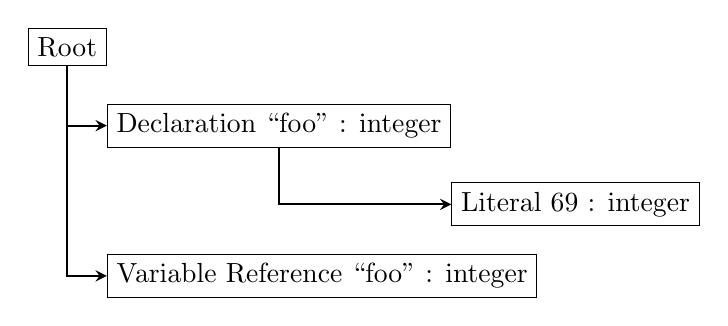
\begin{tikzpicture}
    \node (r) [draw, anchor=west] {Root};

    \node (decl) [draw, below=of r.east, anchor=west] {Declaration ``foo'' : integer};
    \draw [arrow] (r) |- (decl);
    {
      \node (initialiser) [draw, below=of decl.east, anchor=west] {Literal 69 : integer};
      \draw [arrow] (decl) |- (initialiser);
    }

    \node (ref) [draw, below=of decl.west, anchor=west, yshift = -6ex] {Variable Reference ``foo'' : integer};
    \draw [arrow] (r) |- (ref);

  \end{tikzpicture}
  \caption{Node tree produced by parsing tokens from \autoref{fig:int-tokens})}
  \label{fig:int-tree}
\end{figure}

\subsection{Notable Actions}
\label{subsec:node-tree:notable-actions}

\noindent\textbf{Semantic Analysis}\\
Semantic analysis is the act of ensuring a given program is semantically valid. That is, the rules of the program don't contradict each other. For example, this is where type checking is done, as well as ensuring program correctness (i.e. Intercept requires a program return value as the last expression present in a program).

\section{Intermediate Representation (IR)}
\label{sec:ir}

This is where it gets ... compiler-y. Indeed, this is the point at which front-ends hand control flow off to the compiler core/internals. While an AST \emph{is} a truthful representation of a program, it's also very high level: it contains for loops, variable declarations, assignments, and more. The IR has a few simple goals in mind, but all of them are towards the common goal of being as generically optimisable as possible. We want to be able to reduce $2 + 2$ into $4$ without requiring each frontend to write that code, and the IR is the conduit to make that a reality. As each language front-end generates IR, we can apply the same optimisations to any language added to the compiler, greatly reducing code duplication within the compiler codebase \textbf{and} increasing efficiency and speed of output code.

What is passed in from the frontend is regarded as \emph{unlowered} IR. Unlowered IR is an SSA representation of a program that also has a valid control flow graph built into it; this is ideal for optimisations.

After optimisations are applied, the IR is lowered; this is when target triples come into play. Basically, each target may have slightly different semantics/requirements. For example, to lower the IR to fit a specific calling convention, copies to argument registers are often inserted (and stack allocations and corresponding loads/stores). If it doesn't require specific machine instructions to implement, and can be represented by generalised machine instructions like ``load'', ``store'', etc, then it goes here. Mostly calling convention stuff here, but could also be lowering of unaligned accesses and stuff like that, for other arches.

% TODO: What does IR for Intercept example look like?

\subsection{Notable Actions}
\label{subsec:ir:notable-actions}

\noindent\textbf{Optimisation}\\

\noindent\textbf{Target-specific IR Lowering}\\

\section{General Machine IR}
\label{sec:general-machine-ir}

Once the IR is lowered, it is translated (nearly 1:1) into general machine IR (gMIR). Machine IR is in a different format than IR, in that each instruction has an opcode and a variable amount of operands, each of which may have it's own type and value. This differing view on the program allows for pattern matching, as each MIRInstruction contains the types of it's operands within it, and their values, whereas each IRInstruction operand is just a pointer to another IRInstruction.

Because gMIR instructions are only generated from IR instructions, each gMIR instruction still corresponds to an SSA virtual register. Therefore, each gMIR instruction has a ``result'' register that may be used to reference it's value (or really the value that the IR SSA expected to be in that virtual register). To understand this, let's imagine a copy gMIR instruction. It only has a single operand: the thing it's copying. But if it only has one operand, where does it copy to? Well, the copy's destination is the virtual register of the IR instruction it was lowered from.

Another change from IR to gMIR: gMIR keeps track of (stack) frame objects. Each stack allocation will insert an entry into the function's frame objects table corresponding to it's size.

Some types of IRInstruction are removed during generation of gMIR. For example, usages of immediate instructions return an ``inlined operand'', and therefore no machine instruction is required to load an immediate (except for in niche cases with PHI nodes, but we won't get into that).

% TODO: Example, what does gMIR look like?

\subsection{Notable Actions}
\label{subsec:general-machine-ir:notable-actions}

\noindent\textbf{phi2copy}\\
\indent For each function translated, there is a phi2copy pass where PHI instructions are removed, and copies are inserted for each argument into a virtual register.

% TODO: Add a little diagram here with before and after gMIR, PHI'd up and then PHI-less with copies.
\noindent\textbf{Instruction Selection}\\
\indent This is a doozy. It's such a doozy that there is an entire (domain-specific) language built-in to the compiler to accomplish this. But the basics go like this: each supported ISA defines it's own MIR opcodes (separate from the general MIR opcodes). The DSL is then used to write a file containing match/emit patterns, where general MIR instructions with specific patterns of operands are converted into lowered MIR instructions. See \emph{src/codegen/x86\_64/arch\_x86\_64.isel}.

\vspace{1ex}
Example of a simple x86\_64 instruction selection pattern:\\
\indent \indent match MIR\_ADD(Immediate lhs, Register rhs)\\
\indent \indent emit MX64\_ADD(lhs, rhs)
\vspace{1ex}

Now, when an MIR\_ADD with an immediate and then a register operand is found in the general MIR, it will be replaced with a single MX64\_ADD, with the same operands (because x86\_64 has an immediate to register add opcode). This is possibly the simplest pattern, and it gets more and more complex from here. In the future, it would be really nice to be able to ensure two operands have the same value, but I haven't gotten around to writing that into the DSL yet.

\section{Lowered Machine IR}
\label{sec:lowered-machine-ir}

Instruction selection (described in more detail above) converts gMIR into lMIR by using opcodes and operand layouts that the architecture specifically has machine instructions for. However, instruction selection isn't the full picture: almost every backend has some gMIR instructions that have to be lowered in code, and so no patterns are written for them and then after instruction selection has completed, the complex lowering happens of any gMIR opcodes still present. Notoriously, function calls tend to require complex lowering.

After lowering of gMIR, while we \emph{have} made sure every opcode is able to be handled by the target, we haven't done the same to the register operands. There are still a bunch of virtual register operands that don't correspond to hardware registers, so if we tried to just emit code directly after ISel, then we would have a very bad time. This is where (the dreaded) register allocation comes into play.

After register allocation there is a final fixup pass before moving on to actually emit the target code.

% TODO: Example, what does lMIR look like?

\subsection{Notable Actions}
\label{subsec:lowered-machine-ir:notable-actions}

\noindent\textbf{Complex Lowering}\\
\indent Instruction selection isn't able to handle every corner case of every target, so some lowering happens in code vs through pattern matching.

\noindent\textbf{Register Allocation}\\
\indent Register allocation is an NP-complete problem, so you \emph{know} this is going to be good.

To prepare, we calculate defining uses of virtual registers within a function: currently this is a bit hacked, and I don't believe we are setting defining uses \emph{perfectly}. But it's close enough for now. In the future, we would ideally follow control flow of the program to determine a virtual register operands first use. This may produce multiple defining uses, depending on the control flow of the input program (imagine a variable $x$ in virtual register $v1$ that is assigned to $2$ in a then branch and assigned to $3$ in the else branch: in the block that both the then and otherwise branch to, the defining use of virtual register $v1$ depends entirely on which control flow is taken).

Once defining uses of virtual register operands are calculated, we can \emph{actually} get started on RA.

We start by collecting all virtual register operands into a list, and assigning each one an index based on where it is in this list. Basically, each virtual register is enumerated. This means that whenever we encounter a virtual register operand, we can easily find an index that uniquely identifies it: this is crucial for the following steps.

The goal of all of these next steps is to produce an adjacency graph, where each virtual register may either not interfere or interfere with any other virtual register. To interfere means that the two virtual registers have live ranges that overlap, and therefore must not be assigned to the same hardware register.

First, we build an adjacency matrix. This is a lower-left two-dimensional matrix of boolean values defaulting to false, size $N$ by $N$ where $N$ is the number of unique virtual registers collected above. To do this, we walk all paths of control flow, backwards from each function exit all the way to the entry, keeping track of virtual register operands we've seen but not yet seen the defining use of. All virtual register operands used within a single instruction interfere with each other, as well. When two instructions interfere, we set the boolean value in the matrix to true.

Once all control flow paths have been followed, the adjacency matrix is complete. From here, we convert the adjacency matrix into a more useful data structure for what we're about to do: adjacency lists. Each virtual register gets it's own adjacency list. Each adjacency list contains a list of virtual register indices that interfere with the adjacency list's virtual register. This allows us, for each virtual register, to easily visit all other virtual registers that interfere; this is exactly what we want.

With adjacency lists created, we apply a graph-colouring algorithm to the graph, potentially (WIP) spilling registers when we don't have enough colors (a la registers) to properly color it. A lot of functions don't require spilling at all, so it's kind of a corner case.

At this point, each virtual register operand has been coloured, AKA mapped to a hardware register. All that's left is to loop over the instructions and replace all references to virtual registers with references to the hardware register mapped to it. The function gets a bitmask set for each register in use within the function, that way backends can determine which caller/callee saved registers need to be saved/restored, for example.

\noindent\textbf{Final Fixup}\\
\indent While it may seem kind of crazy, there is yet another stage where the lMIR is altered, even after RA. This is for target-specific things like removing register to register moves when the registers are equal, or (final) lowering of calls (i.e. insert saving/restoration of caller-saved registers, if needed).

\section{Target Code}
\label{sec:target-code}

At this point, the lowered MIR is traversed and emitted. What is emitted and how it happens is up to each target.

Currently, x86\_64 architecture supports GNU assembly in both AT\&T and Intel syntax, as well as a GenericObjectFile backend which may be emitted as an ELF or COFF object file.

% TODO: Example, what does output assembly look like?

\end{document}
